\chapter{Forces, Quarks, and the First Hadron Multiplets}

\section{Particles, Fields, and the Missing Third Leg}

Waves are configurations of fields, so the two descriptions are closely related in the present discussion. Quantum mechanics says that the energy in such a wave comes in discrete, indivisible units. Those units are its quanta, and the quanta of a field are what we call its particles. With that relation in hand, we have already discussed wave equations, action principles, and the broad properties carried by particles: energy, momentum, spin, and the boson--fermion distinction. Fermions resist occupying the same state; bosons may congregate and condense into one state.

A quantum Lagrangian also records interactions. Products of fields represent vertices at which particles enter and leave. A term with four powers of a field, for example, represents a four-leg interaction vertex. This is how the action principle becomes a compact inventory of possible particle processes.

The next task is to name the particles---not quite one by one, but in families---and give each some personality: its properties, its interactions, and its place in ordinary physics. Before making that list, however, one side of a conceptual triangle is still missing:
\begin{itemize}
\item particles,
\item fields for which those particles are quanta,
\item forces associated with exchange processes involving those same quanta.
\end{itemize}

The word \emph{elementary} must remain provisional. Every plausible definition of an elementary rather than composite particle eventually encounters a slippery case, and we shall return to that problem. For now, suppose that fundamental fields exist and call their quanta elementary particles. If an electric field gives rise to electric forces and a gravitational field to gravitational forces, then the electron field must also participate in forces. The triangle can close only if force has a particle description as well as a field description.

We shall therefore derive the logic of force twice. First we use classical field energy; then we ask how the same interaction appears when a field is resolved into quanta. Only after that bridge is secure will the particle catalogue begin.

\section{Force from Field Energy in Classical Electrodynamics}

Place two charges in space. One way to find their force is to quote the inverse-square law. A more revealing way is to ask what the charges do to space: they create electric fields, and those fields store energy.

It is useful to separate each charge from the spatial shape of its field,
\begin{equation}
\mathbf E_i=q_i\widehat{\mathbf E}_i,
\end{equation}
although nothing depends on keeping the hat notation. With both charges present, linearity gives
\begin{equation}
\mathbf{E}=\mathbf{E}_1+\mathbf{E}_2.
\end{equation}
Apart from the choice of units, the electrostatic field energy has the form
\begin{equation}
U_{\text{field}}\propto\int d^3x\,\mathbf{E}^2.
\end{equation}
Substituting the sum of the two fields gives
\begin{align}
U_{\text{field}}
&\propto\int d^3x\,(\mathbf{E}_1+\mathbf{E}_2)^2 \\
&\propto\int d^3x\,\bigl(\mathbf{E}_1^2+\mathbf{E}_2^2
  +2\mathbf{E}_1\!\cdot\!\mathbf{E}_2\bigr).
\end{align}

The first two terms are self-energies. Translating either charge moves its field with it and does not change the corresponding integral. That energy contributes, through \(E=mc^2\), to the measured mass of the isolated charged particle. How that self-energy is incorporated into the measured mass belongs to the later subject of renormalization. None of this position-independent energy contributes to the force between the two particles.

The cross-term is different. It belongs to neither particle separately and exists only when both fields are present. If the charges are taken very far apart, their appreciable field regions scarcely overlap. As the charges approach, the overlap changes. The configuration-dependent interaction energy is therefore proportional to
\begin{equation}
U_{\text{int}}(r)\propto q_1q_2\int d^3x\,
\widehat{\mathbf E}_1\!\cdot\!\widehat{\mathbf E}_2.
\end{equation}
For two point charges separated by \(r\), evaluating the integral gives the familiar dependence
\begin{equation}
U_{\text{int}}(r)\propto\frac{q_1q_2}{r}.
\end{equation}
The radial force is its negative gradient,
\begin{equation}
\mathbf F_{12}=-\boldsymbol\nabla_{\mathbf r}U_{\text{int}},
\qquad
|\mathbf F_{12}|\propto\frac{|q_1q_2|}{r^2}.
\end{equation}
\editorialnote{The spoken argument identifies the cross-term with the inverse-square Coulomb force without pausing at the potential. The standard intermediate \(U_{\mathrm{int}}\propto1/r\) is written explicitly here so that its gradient gives the stated \(1/r^2\) force.}

The force law has become the derivative of the part of the field energy that knows about relative position. Far apart, the two objects are effectively independent. Bring them together and the field between them is rearranged; the resulting change in energy is the interaction.

But if a field can be resolved into quanta, this cannot be the end of the story. The same force must have a particle-language account.

\section{Molecular Exchange: Two Protons and One Electron}

Before returning to electrodynamics, consider a system in which exchange is easier to picture: two protons and one electron. Exchange is only one of several origins of molecular forces, but this example makes the relation between exchange, energy, and force visible. It is not offered as a substitute for quantum electrodynamics.

If one proton is present and the other is infinitely far away, the electron may occupy the hydrogenic ground state centered on the first proton. Its wave function is localized near that force center.

\begin{figure}[h]
\centering

\includegraphics[width=0.72\textwidth]{lecture_01_figure_02.png}

\medskip

\begin{tikzpicture}[scale=0.95]
\draw (-0.2,0) -- (6.4,0);
\fill (1.3,0) circle (2pt);
\draw[smooth] plot coordinates {(0.1,0.15) (0.8,1.15) (1.5,1.75) (2.2,1.1) (3.0,0.35) (3.8,0.12)};
\node at (1.3,-0.35) {$p$};
\node at (2.7,1.55) {$\psi_1(x)$};
\end{tikzpicture}
\caption{A hydrogenic ground-state wave function localized near one proton.}
\lectureframe{00:14:32}
\end{figure}
\editorialnote{The label \(\psi_1(x)\) in the redraw names the localized profile described at 00:14:30--00:14:32; it is not copied from a legible board label.}

Now place a second proton at a large but finite separation. By symmetry there is a second localized state with the same one-center energy, this time centered on the right proton.

\begin{figure}[h]
\centering

\includegraphics[width=0.78\textwidth]{lecture_01_figure_03.png}

\medskip

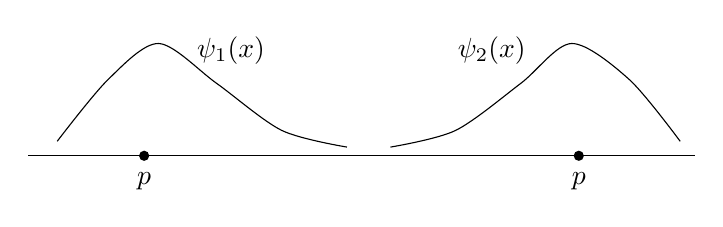
\begin{tikzpicture}[scale=0.92]
\draw (-0.2,0) -- (9.0,0);
\fill (1.4,0) circle (2pt);
\fill (7.4,0) circle (2pt);
\draw[smooth] plot coordinates {(0.2,0.2) (0.9,1.05) (1.6,1.55) (2.4,1.0) (3.3,0.35) (4.2,0.12)};
\draw[smooth] plot coordinates {(4.8,0.12) (5.7,0.35) (6.6,1.0) (7.3,1.55) (8.1,1.05) (8.8,0.2)};
\node at (1.4,-0.35) {$p$};
\node at (7.4,-0.35) {$p$};
\node at (2.6,1.45) {$\psi_1(x)$};
\node at (6.2,1.45) {$\psi_2(x)$};
\end{tikzpicture}
\caption{The two localized profiles used to form the equilibrium superposition after tunneling is allowed.}
\lectureframe{00:17:54}
\end{figure}
\editorialnote{The labels \(\psi_1(x)\) and \(\psi_2(x)\) identify the two profiles discussed at 00:17:41--00:17:56; the symbols are schematic labels added for legibility.}

At infinite separation the two states are degenerate: localizing the electron on the left or on the right costs the same energy. At finite separation a new process becomes possible. The electron can tunnel through the classically forbidden region from one center to the other. Watching for a trajectory through the barrier would disturb the state; ``hopping'' is a description of quantum evolution, not a film of a classical path.

At equilibrium the electron has equal probability of being found near either proton. Normalization therefore supplies the factor \(1/\sqrt2\), and the lower equilibrium state is approximately
\begin{equation}
\psi_+(x)\approx \frac{\psi_1(x)+\psi_2(x)}{\sqrt2}.
\end{equation}

The approximation sign matters. The true two-center wave function is not exactly a sum of two undisturbed hydrogenic orbitals; it adjusts in the overlap region. The point needed here is that the symmetric equilibrium state lies below the isolated one-center energy. In Hamiltonian language, the left and right configurations are coupled by an off-diagonal matrix element. Allowing the electron to occupy their coherent superposition has lowered the energy.

\section{From Lowered Energy to an Effective Force}

At large proton separation the electron-induced contribution \(E_e(r)\) approaches its separated-atom value. At smaller separation, tunneling and superposition lower it. The complete two-proton--one-electron potential must also contain the direct proton repulsion,
\begin{equation}
V_{\mathrm{tot}}(r)=V_{pp}(r)+E_e(r).
\end{equation}

This reconnects the molecular example with the field-energy argument. The wave-function sketches and the qualitative curve for \(E_e(r)\) are two views of the same calculation; equilibrium is determined by the sum \(V_{\mathrm{tot}}(r)\).

\begin{figure}[h]
\centering

\includegraphics[width=0.78\textwidth]{lecture_01_figure_04.png}

\medskip

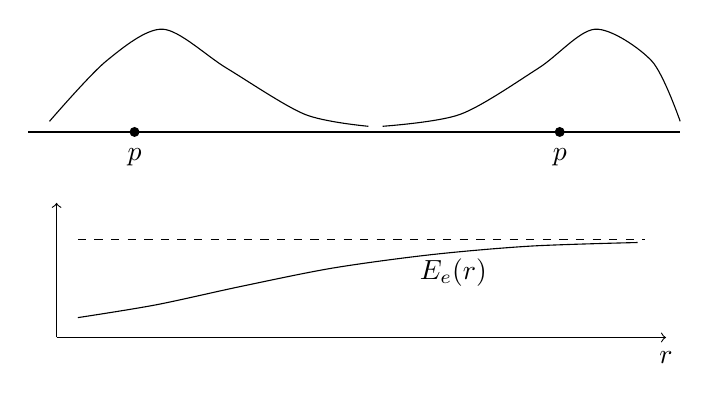
\begin{tikzpicture}[scale=0.9]
\draw (-0.2,3.0) -- (9.0,3.0);
\fill (1.3,3.0) circle (2pt);
\fill (7.3,3.0) circle (2pt);
\draw[smooth] plot coordinates {(0.1,3.15) (0.9,4.0) (1.7,4.45) (2.6,3.9) (3.7,3.25) (4.6,3.08)};
\draw[smooth] plot coordinates {(4.8,3.08) (5.9,3.25) (7.0,3.9) (7.8,4.45) (8.6,4.0) (9.0,3.15)};
\node at (1.3,2.65) {$p$};
\node at (7.3,2.65) {$p$};

\draw[->] (0.2,0.1) -- (0.2,2.0);
\draw[->] (0.2,0.1) -- (8.8,0.1);
\draw[dashed] (0.5,1.48) -- (8.5,1.48);
\draw[smooth] plot coordinates {(0.5,0.38) (1.6,0.56) (2.8,0.82) (4.1,1.08) (5.5,1.27) (6.9,1.39) (8.4,1.44)};
\node at (5.8,1.02) {$E_e(r)$};
\node at (8.8,-0.18) {$r$};
\end{tikzpicture}
\caption{Wave-function overlap above and the electron-induced energy below. It rises toward the separated-atom asymptote as \(r\) increases; the total proton potential must also include their Coulomb repulsion.}
\lectureframe{00:20:28}
\end{figure}
\editorialnote{The labels \(E_e(r)\) and \(r\) identify the energy curve and separation discussed at 00:19:12--00:20:38; the surviving board frame does not make those axis labels legible.}

The two corresponding forces follow from the energy gradients,
\begin{equation}
F_{e}(r)=-\frac{dE_e}{dr},
\qquad
F_{\mathrm{tot}}(r)=-\frac{dV_{\mathrm{tot}}}{dr}.
\end{equation}
The system is therefore pushed toward lower total energy. Where \(E_e(r)\) decreases as the protons approach, exchange supplies an attractive contribution; whether a bound separation exists depends on its competition with \(V_{pp}(r)\). This is the elementary mechanism behind a covalent bond: the electron is shared because the shared state is energetically favorable.

In the classical calculation, overlap of electric fields changes the energy. Here, two force centers allow a lower quantum state. Both mechanisms produce force because the equilibrium energy depends on configuration.

The exchange language may be summarized by a worldline sketch. It must not be read as an observed trajectory; it represents amplitudes for the electron to be associated with either proton.

\begin{figure}[h]
\centering
\begin{tikzpicture}[scale=1.0]
\draw (0,0) -- (0,4.4);
\draw (4.8,0) -- (4.8,4.4);
\draw (0,0.9) .. controls (1.6,1.7) and (3.2,1.7) .. (4.8,2.5);
\draw (4.8,2.9) .. controls (3.2,2.1) and (1.6,2.1) .. (0,3.9);
\node at (0,-0.35) {$p$};
\node at (4.8,-0.35) {$p$};
\node at (2.35,1.55) {$e^-$};
\node at (2.35,2.55) {$e^-$};
\end{tikzpicture}
\caption{Electron exchange between two proton worldlines, understood as a schematic of quantum amplitudes rather than a watched path.}
\end{figure}

\begin{classroomqa}
\audiencequestion{Can the attraction be understood simply as the electron screening or reducing the proton charge?\lecturetimestamp{00:23:26}}
\lecturerresponse{No. Charge reduction is not the right picture for this effect. The essential fact is that adding the two localized wave functions produces a state with slightly lower energy than either localized state separately.}
\end{classroomqa}

\begin{classroomqa}
\audiencequestion{Is this what Feynman meant by saying that ``light likes light''?\lecturetimestamp{00:23:51}}
\lecturerresponse{No. That phrase most likely concerns Bose statistics: photons favor common states, whereas electrons obey exclusion. The molecular effect here is tunneling between two centers.}
\end{classroomqa}

The two protons still repel electrostatically. Exchange is shorter-ranged than the Coulomb interaction, so the total potential must be considered rather than either contribution alone. At appropriate separations the molecular ion \(\mathrm H_2^+\) is nevertheless bound; in a neutral two-electron system the long-range charge repulsion is absent and covalent binding is even more familiar.

\begin{classroomqa}
\audiencequestion{Does placing the electron between the protons mainly reduce their electrostatic repulsion?\lecturetimestamp{00:24:33}}
\lecturerresponse{It reduces the repulsion a little, but that is not the main effect. Electron exchange is a shorter-range force than the Coulomb repulsion. It is most visible in a neutral two-electron system, where the long-range electrostatic force between the atoms is absent but tunneling still produces an attraction.}
\end{classroomqa}

\begin{classroomqa}
\audiencequestion{Is the positively charged molecular ion \(\mathrm H_2^+\), with only one electron, actually bound?\lecturetimestamp{00:26:06}}
\lecturerresponse{Yes. At sufficiently small separation the exchange attraction is strong enough to overcome the proton--proton Coulomb repulsion.}
\end{classroomqa}

\begin{classroomqa}
\audiencequestion{Does the two-center arrangement create a third force?\lecturetimestamp{00:26:24}}
\lecturerresponse{No new fundamental force is introduced. The Schr\"odinger equation in the combined potential of the two protons has an equilibrium energy different from the one-center problem; the derivative of that changed energy is the effective force.}
\end{classroomqa}

\begin{classroomqa}
\audiencequestion{Is the energy lowering an example of quantum entanglement?\lecturetimestamp{00:27:06}}
\lecturerresponse{Not in the ordinary two-particle sense: only one electron is required. The relevant mathematical feature is an off-diagonal Hamiltonian matrix element coupling the left and right states.}
\end{classroomqa}

\begin{classroomqa}
\audiencequestion{What happens to the exchange at high temperature?\lecturetimestamp{00:27:37}}
\lecturerresponse{At extreme temperature the electron is ionized and forgets the molecule altogether. At a lower excitation energy it may occupy a larger orbital, changing the overlap and hence the force. This is a state-dependent correction, not a new general mechanism.}
\end{classroomqa}

\section{Photon Exchange and the First Entries of the Table}

Can the Coulomb force be told in the same exchange language? A charged particle interacts with the electromagnetic field, whose quanta are photons. Classically we solve for the electric field around the charge. In quantum field theory we resolve that interaction into photon emission and absorption.

A physical charged particle is not merely a bare charge. Its state is a quantum superposition containing a bare electron component, an electron with one photon, an electron with two photons, and so on. In deliberately schematic notation,
\begin{equation}
\begin{aligned}
\ket{e_{\mathrm{phys}}}
={}&a_0\ket e
+a_1\ket{e+\text{one photon}}
\\
&+a_2\ket{e+\text{two photons}}+\cdots .
\end{aligned}
\end{equation}
This notation records only the hierarchy of photon-number components; it does not specify photon momenta or attempt a complete construction of an interacting charged state.
The surrounding photons are emitted and reabsorbed rather than escaping as free radiation. Their effects can be measured, although they are not detected in the same way as freely propagating photons. Put a second charge nearby and a photon emitted at one charge can be absorbed at the other. The two dressed states then cease to have an energy equal to the simple sum of two isolated energies.

The classroom analogy is two jugglers, each handling a set of balls. When they are far apart, each juggles independently. Bring them close enough and one may catch a ball thrown by the other. In the Feynman-diagram language, that shared object is the exchanged photon. The analogy is not a microscopic trajectory, but it captures why proximity permits a new process.

We now have two descriptions beyond merely memorizing Coulomb's law. Classical field theory adds the fields and squares the result. Quantum field theory sums amplitudes in which quanta are exchanged. Particles, fields, and forces form a one-to-one-to-one correspondence in this sense. Electrons mediate molecular exchange, photons mediate electromagnetic exchange, and any particle that can be exchanged can contribute to a force in an appropriate setting. Thus the familiar statement that nature has four fundamental interactions is a classification at a broader level; within exchange language, each exchangeable species can generate its own effective force contribution.

It is finally time to name the particles, list their properties, and say which processes they can enter. Writing the entire Standard Model at once would only produce a long memory test, so we shall divide the particles into small groups whose members are simply related and learn what each group can do.

The full catalogue is cumbersome because we do not understand why precisely these particles exist while other imaginable particles do not. Mathematical consistency supplies some relations: once several members of a pattern exist, another may be required to complete it. Those relations reduce the number of independent facts, but only by a modest factor. Many particle types and many parameters remain unexplained. Understanding that unfinished structure is necessary for understanding what later experiments are trying to discover.

\begin{figure}[h]
\centering

\includegraphics[width=0.7\textwidth]{lecture_01_figure_05.png}
\caption{The first particle-table entry identifies the photon by \(\gamma\) and its field by the vector potential \(A\).}
\lectureframe{00:39:11}
\end{figure}

The first field--quantum identification is
\begin{equation}
\gamma \leftrightarrow A.
\end{equation}
Here \(A\) is the electromagnetic vector potential. The photon is a spin-one boson with zero electric charge, zero baryon number, and zero rest mass. The electron field is conventionally denoted \(\psi_e\); its creation and annihilation pieces act on electron and positron states.

Our table records the name, particle symbol, field, boson or fermion type, electric charge \(Q\), baryon number \(B\), and mass:

\begin{table}[h]
\centering
\resizebox{\linewidth}{!}{%
\begin{tabular}{lllllll}
Name & Symbol & Field & Type & \(Q\) & \(B\) & Mass \\
Photon & \(\gamma\) & \(A\) & boson & \(0\) & \(0\) & \(0\) \\
Electron & \(e^-\) & \(\psi_e\) & fermion & \(-1\) & \(0\) & \(0.51\,\mathrm{MeV}\) \\
Positron & \(e^+\) & \(\psi_e\) & fermion & \(+1\) & \(0\) & \(0.51\,\mathrm{MeV}\)
\end{tabular}
}%
\caption{The photon and electron--positron entries that begin the particle catalogue.}
\end{table}

The relation between electron and positron is mutual: each is the antiparticle of the other. Calling the negatively charged state ``the particle'' is convention. We measure electric charge in units of the magnitude of the electron charge, so
\begin{equation}
Q(e^-)=-1,\qquad Q(e^+)=+1.
\end{equation}
Mass is measured in energy units by using \(E=mc^2\). One electron volt is the energy acquired by a charge \(e\) through a potential difference of one volt,
\begin{equation}
1\,\mathrm{eV}=e\,(1\,\mathrm V).
\end{equation}
The unit comes naturally from atomic physics: as a rough atomic scale, ionizing hydrogen costs about \(13.5\,\mathrm{eV}\). Particle masses require millions or billions of electron volts. The electron mass is
\begin{equation}
m_e c^2 \approx 0.511\,\mathrm{MeV}.
\end{equation}

\begin{classroomqa}
\audiencequestion{Should the electron mass be exactly one half of an MeV?\lecturetimestamp{00:44:02}}
\lecturerresponse{No. The convenient rounded value \(0.51\,\mathrm{MeV}\) is not fixed to an exact half by any principle; it is a measured parameter.}
\end{classroomqa}

The elementary QED process has one charged-fermion line entering, one leaving, and one photon line attached. Rearranging or crossing the legs lets the same vertex describe photon emission, absorption, or a positron process. In the noncovariant schematic notation used here, the interaction contains
\begin{equation}
\mathcal{L}_{\mathrm{int}}\sim e\,\psi_e^\dagger \psi_e A.
\end{equation}
Expanding the fields into creation and annihilation operators produces terms that remove an incoming electron, create an outgoing electron, and create or annihilate a photon. The coupling \(e\) supplies one factor at the vertex. Thus, for photon emission while an electron is scattered or accelerated,
\begin{equation}
\mathcal{A}_{\mathrm{vertex}}\propto e,
\qquad
P_{\mathrm{emission}}\propto e^2.
\end{equation}
An electron striking the target in an X-ray tube is one practical setting in which this photon-emission probability matters. Repeated combinations of the same vertex generate the processes of quantum electrodynamics, including the energy shift interpreted as the force between charges.

A schematic vertex is therefore useful.

\begin{figure}[h]
\centering
\begin{tikzpicture}[scale=1.0]
\fill (0,0) circle (1.5pt);
\draw (-1.6,-1.2) -- (0,0) -- (1.6,-1.2);
\draw (0,0) -- (0,1.8);
\node at (-1.8,-1.4) {$e^-$};
\node at (1.8,-1.4) {$e^-$};
\node at (0.35,1.95) {$\gamma$};
\end{tikzpicture}
\caption{Topological schematic of the elementary QED vertex: one charged-fermion line enters, one leaves, and one photon is attached. The straight photon leg is only a simplified drawing convention here.}
\end{figure}

The exchange contribution to the force joins two such vertices:

\begin{figure}[h]
\centering
\begin{tikzpicture}[scale=1.0]
\draw (0,0) -- (0,4.0);
\draw (4.8,0) -- (4.8,4.0);
\draw (0,2.0) -- (4.8,2.0);
\node at (0,-0.35) {$e^-$};
\node at (4.8,-0.35) {$e^-$};
\node at (2.4,2.3) {$\gamma$};
\end{tikzpicture}
\caption{Topological schematic of photon exchange, giving the quantum-field-theoretic description of the Coulomb interaction.}
\end{figure}

With the particle--field--force triangle closed, we can continue the catalogue.

\section{Quarks, Baryon Number, and the Puzzle of Families}

Had this catalogue been written around 1960, protons and neutrons would probably have followed electrons and photons. Modern particle physics inserts quarks first. In the naive constituent picture, protons and neutrons are comparatively large composites made from smaller quark degrees of freedom. The exact meaning of \emph{composite} remains to be examined, but the constituent language is already enormously useful.

All quarks are fermions. They carry baryon number, a quantity introduced in nuclear physics by counting nucleons. A \emph{nucleon} means specifically a proton or neutron. A \emph{baryon} is the broader class that contains nucleons and the similar heavy particles encountered later. A proton and a neutron each have one unit,
\begin{equation}
B(p)=B(n)=1,
\qquad
B(\bar p)=B(\bar n)=-1.
\end{equation}
For a nucleus, this baryon count is exactly the mass number \(A=Z+N\), the number of protons plus neutrons. The numerical atomic mass measured in atomic-mass units is only approximately \(A\). Protons may turn into neutrons and neutrons into protons in beta processes, but the total number of nucleons is unchanged. For example,
\begin{equation}
n\longrightarrow p+e^-+\bar\nu_e
\end{equation}
changes the proton and neutron counts separately while preserving their sum.

\begin{classroomqa}
\audiencequestion{Do isotopes contradict conservation of proton number plus neutron number?\lecturetimestamp{00:52:03}}
\lecturerresponse{Different isotopes do contain different neutron numbers, and beta decay can interchange a neutron and a proton. In an ordinary nuclear process the relevant conserved count is the total baryon number, not either species separately.}
\end{classroomqa}

The normalization is conventional. We might have assigned a proton baryon number \(2\), \(7\), or \(\pi\), provided every composite scaled consistently. Once the proton is assigned \(B=1\) and contains three quarks, each quark must carry
\begin{equation}
B(q)=\frac13,
\qquad
B(\bar q)=-\frac13.
\end{equation}
The fractional value is therefore a historical consequence of normalizing the composite nucleon first.

\begin{classroomqa}
\audiencequestion{Is the number of quarks conserved?\lecturetimestamp{00:54:23}}
\lecturerresponse{Quark--antiquark pairs may be created or destroyed, so the raw number is not conserved. The quantity corresponding to baryon number is the number of quarks minus antiquarks, divided by three. Empirically it is conserved to extremely high accuracy, although it is not assumed here to be an absolute law.}
\end{classroomqa}

A hypothetical charge-conserving decay such as
\begin{equation}
p\longrightarrow e^++\gamma
\end{equation}
would carry baryon number one into a final state with baryon number zero. The channel is an illustrative bookkeeping example, not a proposed decay model. No baryon-number-violating process has been observed. The rough bound quoted here puts the proton lifetime at least in the range of \(10^{33}\)--\(10^{34}\) years. One does not watch a single proton for that long; one watches an enormous number of protons for a manageable time, trading lifetime against sample size. Proton decay was nevertheless widely expected, and nothing in the mathematics being discussed here supplied an absolute prohibition. Whether baryon number is exact therefore remained an open experimental question: unobserved, strongly constrained, but not dismissed.

\begin{classroomqa}
\audiencequestion{Does proton--antiproton annihilation violate baryon number?\lecturetimestamp{00:56:17}}
\lecturerresponse{No. The initial baryon number is \(1+(-1)=0\), so annihilation into a zero-baryon-number final state conserves it. A lone proton decaying to nonbaryonic products would be the violation.}
\end{classroomqa}

There are six quark flavors,
\begin{equation}
u,\ d,\ s,\ c,\ b,\ t,
\end{equation}
called up, down, strange, charm, bottom, and top. Nothing points upward about an up quark, and a strange quark is no stranger than its neighbors; the names record history rather than logic. Field notation is not perfectly uniform: one encounters \(q\), \(Q\), \(\psi_q\), or simply the flavor letter \(u,d,s,c,b,t\) for both the field and its quantum.

\begin{classroomqa}
\audiencequestion{Are bottom and top the same particles that were once called beauty and truth?\lecturetimestamp{00:58:35}}
\lecturerresponse{Yes. The less ornate names bottom and top became standard. The naming history carries no dynamical content.}
\end{classroomqa}

Their electric charges repeat in three pairs:
\begin{equation}
\begin{aligned}
Q(u)=Q(c)=Q(t)&=+\frac23,
\\
Q(d)=Q(s)=Q(b)&=-\frac13.
\end{aligned}
\end{equation}
Antiquarks carry the opposite charges and baryon number. Isolated fractional charge is never seen because quarks do not occur as free asymptotic particles; observed hadrons have integer electric charge.

The pairs \((d,u)\), \((s,c)\), and \((b,t)\) are three families repeating the same charge pattern. All six still carry \(B=1/3\).

\begin{classroomqa}
\audiencequestion{Do the heavier quarks also carry baryon number \(1/3\)?\lecturetimestamp{01:02:02}}
\lecturerresponse{Yes. Every quark carries baryon number \(1/3\).}
\end{classroomqa}

The masses show no comparable repetition. Useful order-of-magnitude values are
\begin{align}
m_u &\sim 5\,\mathrm{MeV},
&
m_d &\sim 10\,\mathrm{MeV},
\\
m_s &\sim 100\,\mathrm{MeV},
&
m_c &\sim 10^3\,\mathrm{MeV},
\\
m_b &\sim 5\,\mathrm{GeV},
&
m_t &\sim 170\,\mathrm{GeV}.
\end{align}
Here \(1\,\mathrm{GeV}=10^3\,\mathrm{MeV}\); the change of unit keeps the bottom- and top-quark entries readable. The down-quark estimate is far above the electron's \(0.511\,\mathrm{MeV}\) but far below the proton's roughly \(940\,\mathrm{MeV}\), about \(1{,}800\) electron masses. Indeed, adding two light up-quark entries and one down-quark entry does not come close to the proton mass; the rest of the hadron's energy must eventually be accounted for.

\editorialnote{The spoken comparison called a \(10\,\mathrm{MeV}\) down quark about fifty electron masses. With the rough values written here, \(10/0.511\approx20\); the hierarchy is correct, but the factor fifty is an arithmetic slip.}

Even the ordering within a pair is not repeated: the down quark is heavier than the up, whereas the charm is much heavier than the strange. The top is tens of thousands of times heavier than the up quark, even though their charges and interaction pattern are closely analogous.

There are really two puzzles here. We do not understand why even one quark family exists, although the first family at least supplies the up and down quarks needed for protons, neutrons, and ordinary matter. Nor do we understand why nature repeats that pattern in a second and a third family, or why the repeated particles have masses scattered over so many orders of magnitude. There are ideas, but no accepted explanation that calculates this pattern.

\begin{classroomqa}
\audiencequestion{If the top-quark mass has no fundamental explanation, how was its approximate value anticipated before direct discovery?\lecturetimestamp{01:05:53}}
\lecturerresponse{The estimate did not derive the mass from a deeper principle. One assumes a candidate mass, computes diagrams in which virtual top quarks affect well-measured processes, and asks which value is consistent with those observations. Indirect sensitivity can locate a parameter without explaining why nature chose it.}
\end{classroomqa}

\begin{classroomqa}
\audiencequestion{If a free quark cannot be isolated, in what sense can a quark be detected?\lecturetimestamp{01:08:04}}
\lecturerresponse{Evidence for quarks is detectable: their production leaves characteristic energies, directions, and particle jets, and virtual quarks affect other observables. What cannot be prepared is a lone quark separated from all hadronic companions and examined as an isolated asymptotic particle.}
\end{classroomqa}

\begin{classroomqa}
\audiencequestion{Is the pattern of charges \(-1/3\) and \(+2/3\) derived from theory or merely bookkeeping?\lecturetimestamp{01:09:02}}
\lecturerresponse{Some of the pattern is required by mathematical consistency, but only some. At this stage the charges are being recorded as facts; the consistency conditions will be discussed only after more of the Standard Model is in place.}
\end{classroomqa}

Only \(u\) and \(d\) quarks have appreciable abundance in ordinary matter. The heavier flavors decay toward lighter states. The relative abundance of up and down quarks is therefore determined largely by the cosmic and nuclear abundance of protons and neutrons and by their constituent content.

\begin{classroomqa}
\audiencequestion{What determines the relative abundance of the six quark flavors in the universe?\lecturetimestamp{01:09:49}}
\lecturerresponse{Stable matter contains essentially up and down quarks; the heavier flavors decay. Free neutrons decay while protons are stable on observed timescales, although neutrons remain abundant when bound in nuclei. Counting up and down quarks then reduces, at this level, to counting those protons and neutrons.}
\end{classroomqa}

\section{From Quarks to Hadrons: Nucleons, Strange Baryons, and Mesons}

Once the quark charges are known, familiar hadrons can be rebuilt. A neutron and a proton each contain three valence quarks,
\begin{equation}
n=ddu,
\qquad
p=uud.
\end{equation}
Their charges check immediately:
\begin{align}
Q(n) &= Q(d)+Q(d)+Q(u)
= -\frac13-\frac13+\frac23
=0,\\
Q(p) &= Q(u)+Q(u)+Q(d)
= \frac23+\frac23-\frac13
=1.
\end{align}

Forget photons for a moment. With electromagnetism switched off, proton and neutron look almost like the same object with \(u\) and \(d\) interchanged. This near-symmetry is not exact because the two quarks do not have exactly equal masses. We shall name and develop the symmetry only after meeting the corresponding light mesons.

Since \(m_d>m_u\), the neutron, which contains two down quarks, should receive the larger quark-mass contribution. Electromagnetic self-energy pushes in the opposite direction: a charged proton stores electric-field energy, while a neutron has no net charge. Nature resolves the competition with a slightly heavier neutron. At this rough level of approximation,
\begin{align}
m_pc^2&\approx940\,\mathrm{MeV},\\
m_nc^2&\approx940\,\mathrm{MeV},\\
(m_n-m_p)c^2&\approx1.4\,\mathrm{MeV}.
\end{align}

\begin{classroomqa}
\audiencequestion{What are the proton and neutron masses?\lecturetimestamp{01:15:35}}
\lecturerresponse{Both are near \(940\,\mathrm{MeV}\), with a difference of about \(1.4\,\mathrm{MeV}\) at this rough level.}
\end{classroomqa}

That small excess is nevertheless enough to permit free-neutron decay. After paying the electron rest energy, the remaining energy can appear as kinetic energy in \(n\to p+e^-+\bar\nu_e\).

The same constituent logic produces strange baryons. Since \(s\) and \(d\) have the same electric charge, a down quark may be replaced by a strange quark without changing the charge pattern:
\begin{equation}
uds,\qquad uss,\qquad uus.
\end{equation}
Thus \(uds\) and \(uss\) are neutral in the examples above, while \(uus\) has charge \(+1\). Such states received names including \(\Lambda\) and \(\Xi\); no detailed assignment of those names is needed at this stage. Replacing \(d\) by \(s\) is qualitatively analogous to substituting one nucleon species for the other in a related nucleus: much of the binding pattern remains, while the constituent change shifts the mass. These states are heavier than ordinary nucleons and decay to lighter baryons together with whatever additional particles are required to carry energy and the other conserved quantum numbers.

\begin{classroomqa}
\audiencequestion{What appears when a strange baryon decays?\lecturetimestamp{01:19:02}}
\lecturerresponse{A lighter baryon such as a proton or neutron appears, but it cannot be the only product: the excess energy and conserved quantum numbers require additional particles. The detailed decay rules are deferred.}
\end{classroomqa}

The detailed replacement rules are more complicated than this first catalogue, but one safe operation is to replace a flavor by another flavor with the same electric charge. Replacing a down quark by a strange quark adds roughly \(90\,\mathrm{MeV}\) at this rough constituent level. These baryons are therefore somewhat heavier than protons and neutrons. Because they can decay to the lighter nucleons, they are not abundant in ordinary matter or in the cosmos around us.

\begin{classroomqa}
\audiencequestion{Does every baryon have an antibaryon made by replacing each quark with its antiquark?\lecturetimestamp{01:20:33}}
\lecturerresponse{Yes. Replacing every constituent by its antiparticle produces the antiproton, antineutron, or corresponding antistrange baryon, with all additive charges reversed.}
\end{classroomqa}

\begin{classroomqa}
\audiencequestion{What if a strange quark is replaced by a bottom quark instead?\lecturetimestamp{01:21:00}}
\lecturerresponse{The result is a bottom baryon. ``Strange baryon'' specifically means that an \(s\) quark is present; the adjective names the flavor, not a general degree of unfamiliarity.}
\end{classroomqa}

The adjective \emph{strange} arose after physicists had become familiar with protons and neutrons and newly discovered particles seemed unexpected beside them. Once the flavor structure is known, their existence is no stranger than that of any other quark composite.

The constituent masses expose an important warning. Adding two up-quark masses and one down-quark mass gives only a few tens of MeV, nowhere near the proton's roughly \(940\,\mathrm{MeV}\). Something substantial is missing from that naive sum. The proton and neutron also contain gluons, and gluons carry energy. In a relativistic bound system the mass of the composite is not obtained by simply adding the listed masses of its constituents.

\begin{classroomqa}
\audiencequestion{Where does the apparently missing proton and neutron mass come from? Do gluons carry mass?\lecturetimestamp{01:21:26}}
\lecturerresponse{Gluons carry no baryon number in this bookkeeping, but they do carry energy. Their energy is part of why the mass of the proton or neutron is not the sum of the light-quark mass entries.}
\end{classroomqa}

\begin{classroomqa}
\audiencequestion{Is that missing contribution a form of binding energy?\lecturetimestamp{01:22:03}}
\lecturerresponse{Yes, it may be called a form of binding energy. The warning is that relativistic composite masses do not add in the simple way suggested by adding constituent mass parameters.}
\end{classroomqa}

\begin{classroomqa}
\audiencequestion{Can a composite proton be described in field language as well as particle language?\lecturetimestamp{01:22:45}}
\lecturerresponse{Yes, but it is much harder. For the constituent bookkeeping being developed here, particle language is far more transparent than trying to combine the spatially extended fields directly.}
\end{classroomqa}

\begin{classroomqa}
\audiencequestion{Ordinary binding energy is negative relative to separated constituents. Why is the nucleon's dynamical contribution a large positive energy?\lecturetimestamp{01:23:32}}
\lecturerresponse{The usual negative-binding intuition is not true in this case. The explanation belongs to the later treatment of the strong interaction, so for now the question is deferred.}
\end{classroomqa}

Why do three quarks form baryons while two quarks do not form an isolated two-quark hadron? In the early days of quark theory this was a genuine puzzle. One might answer that the observed bound combinations must have electric charge equal to an integer multiple of the electron charge. By itself that sounds circular: it describes the pattern without explaining it. Nevertheless, the rule proved to be pointing in the right direction, and its deeper origin can be understood only after more of the strong interaction is in place. For now it is explicitly a working rule: three quarks can make a baryon, while a quark and an antiquark can make a meson, and the resulting observed composites have integer charge.

Baryons made from three identical light flavors also occur, but their details can wait until after the mesons.

Mesons are \(q\bar q\) composites. Their baryon number vanishes,
\begin{equation}
B(q\bar q)=\frac13-\frac13=0.
\end{equation}
The lightest examples use \(u\) and \(d\). These flavors are much lighter than the others, are stable or comparatively slow to disappear in ordinary matter, and are abundant in nature. Their low production threshold also means that collisions make them more readily than heavy flavors. For all these reasons, light-quark composites were the first mesons encountered experimentally and are the natural place to begin.

The natural flavor basis is
\begin{equation}
\ket{\bar u d},\qquad \ket{u\bar d},\qquad \ket{\bar u u},\qquad \ket{\bar d d}.
\end{equation}
No additional restriction is used in this first count: all four light quark--antiquark pairings are retained, and their electric charges are then computed.

The charged states are immediate. Since \(Q(\bar u)=-2/3\) and \(Q(d)=-1/3\),
\begin{align}
Q(\bar u d)&=-\frac23-\frac13=-1,
&
\ket{\pi^-}&=\ket{\bar u d}.
\end{align}
Replacing every constituent by its antiparticle gives \(u\bar d\), so the second state is the antiparticle of the first:
\begin{align}
Q(u\bar d)&=+\frac23+\frac13=+1,
&
\ket{\pi^+}&=\ket{u\bar d}.
\end{align}

The same-flavor states are neutral, but neither receives a separate particle name by itself. Quantum mechanics permits us to superpose them. The two normalized, orthogonal combinations are
\begin{align}
\ket{\pi^0} &\approx \frac{\ket{\bar u u}-\ket{\bar d d}}{\sqrt2},\\
\ket{\eta} &\approx \frac{\ket{\bar u u}+\ket{\bar d d}}{\sqrt2}.
\end{align}

\begin{figure}[h]
\centering

\includegraphics[width=0.82\textwidth]{lecture_01_figure_06.png}
\caption{The symmetric neutral combination is identified with the \(\eta\), while the antisymmetric combination is grouped with the pion triplet.}
\lectureframe{01:32:35}
\end{figure}

Each neutral state is an entangled quark--antiquark pair, not through ordinary spin but through \emph{upness} and \emph{downness}. If up and down flavor are treated mathematically like the two directions of a spin-half variable, then the sum and difference above play the same role as familiar two-spin superpositions. This internal analogue of spin is called \emph{isospin}. Nothing is literally pointing upward or downward in space; the two directions label \(u\) and \(d\) flavor.

The three pions \(\pi^+\), \(\pi^0\), and \(\pi^-\) form an isospin triplet. Their masses are nearly equal and would coincide more closely if the up and down quarks had exactly the same mass. The orthogonal neutral state is called the \(\eta\).

The \(\eta\) is substantially heavier than a pion:
\begin{equation}
m_\pi \approx 140\,\mathrm{MeV},
\qquad
m_\eta \approx 500\,\mathrm{MeV}.
\end{equation}
Why the \(\eta\) stands apart was obscure for a long time. The explanation is now understood, but it is mathematically abstract and is not developed here.

\begin{classroomqa}
\audiencequestion{Are these mesons relatively long-lived?\lecturetimestamp{01:33:59}}
\lecturerresponse{Relative to many strongly decaying particles, yes. They do not decay through the strong interaction in the channels under discussion; weak and electromagnetic decays make them longer-lived.}
\end{classroomqa}

\begin{classroomqa}
\audiencequestion{Do the individual neutral states \(\bar u u\) and \(\bar d d\) have names of their own?\lecturetimestamp{01:34:29}}
\lecturerresponse{No. The named particles are the linear combinations formed by their sum and difference; those combinations have definite values.}
\end{classroomqa}

\begin{classroomqa}
\audiencequestion{Is this neutral-state superposition like neutrino oscillation?\lecturetimestamp{01:34:44}}
\lecturerresponse{It is similar in the limited sense that both involve quantum superpositions. Here the issue is more closely related to the spin combinations of two spin-half constituents and the two ways such states can be entangled. That discussion is deferred to the next lecture.}
\end{classroomqa}

Once the strange quark is admitted, replacing \(d\) or \(\bar d\) by \(s\) or \(\bar s\) gives the four strange or \(K\)-meson flavor states
\begin{equation}
\bar u s,\qquad u\bar s,\qquad \bar d s,\qquad d\bar s.
\end{equation}
Their charge assignments are
\begin{align}
Q(\bar u s) &=-1,
&
Q(u\bar s) &=+1,
\\
Q(\bar d s) &=0,
&
Q(d\bar s) &=0.
\end{align}
There are therefore two charged and two neutral kaons.

The first count gives three pions, four kaons, and one \(\eta\): eight states. But the list has not yet used the \(\ket{s\bar s}\) pairing. With three flavors and three antiflavors, the complete elementary count is therefore
\begin{equation}
3\times3=9.
\end{equation}
The missing \(s\bar s\) state completes the count of nine quark--antiquark flavor combinations.
